
%(BEGIN_QUESTION)
% Copyright 2010, Tony R. Kuphaldt, released under the Creative Commons Attribution License (v 1.0)
% This means you may do almost anything with this work of mine, so long as you give me proper credit

{\it Ethernet} is a popular communications standard for many digital devices, personal computers included.  Originally, Ethernet was intended to be a network standard for conveying digital data only, without power.  In later years, however, upgrades to the standard allowed DC power to be conveyed over the same wire pairs.  The IEEE standard {\tt 802.3af} is one example of a power-over-Ethernet standard.

Shown here is a schematic showing how two Ethernet devices connect together over a Category 5 ("Cat 5") twisted-pair cable, with DC power conveyed over the same wire pair:

$$\includegraphics[width=15.5cm]{i02289x02.eps}$$

Explain what function(s) the transformers provide in this system, and how they allow DC power to travel through the wire pairs from source to load without interfering with the Ethernet data signals, which are AC.


\vfil

\underbar{file i02289}
\eject
%(END_QUESTION)





%(BEGIN_ANSWER)

This is a graded question -- no answers or hints given!

%(END_ANSWER)





%(BEGIN_NOTES)

The transformers allow the AC (data) signals to be coupled from transmitter to receiver without interference from the DC power source.  Just how it accomplishes this feat is worthy of note.

\vskip 10pt

AC signals are coupled between primary and secondary windings at each transformers, so that the transmitters and receivers may send Manchester-encoded data to one another easily.  The DC power, however, passes in ``split'' fashion through one winding of each transformer so as to provide an unbroken copper path for DC current from source to load.  Trace the DC current from source to load and you will see that there is zero net magnetic flux in the transformer cores resulting from the DC, meaning that the transformers do not ``see'' the DC current for all practical purposes.

\vskip 10pt

What this means is that the DC power cannot interfere with the AC Ethernet signals, even if the DC power happens to pulse or surge.  Most students, looking at the transformers and remembering that only AC can pass through a transformer (and not DC), think this is the principle of design exploited here.  Actually, it's a lot more clever than that!  The fundamental principle of operation here is that the power is routed through the center-tapped winding of each transformer so as to cancel any magnetism it might otherwise produce in each transformer core.  The fact that the power here is DC rather than AC is actually irrelevant!  For the sake of discussion, we could route {\it AC} power the same way and it would have no impact on the Ethernet signals.


%INDEX% Networking, Ethernet: power over Ethernet

%(END_NOTES)


